\documentclass[border=2mm]{standalone}
\usepackage{tikz}
\begin{document}

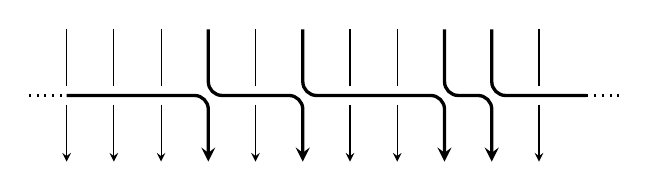
\begin{tikzpicture}[scale=1.2]

% Left extension (dotted)
\draw[thick,dotted] (-0.9,0)--(-0.5,0);

% Leftmost simple vertical line with downward arrow
\draw (-0.5,0.7)--(-0.5,0.1); 
\draw[->,>=stealth] (-0.5,-0.1)--(-0.5,-0.7);

% First thick bent arrow (from x=0 to x=1, then down)
\draw[very thick,rounded corners=5,->,>=stealth] (-0.5,0)--(1,0) -- (1,-0.7);

% Simple vertical lines at x = 0, 0.5
\draw (0,0.7)--(0,0.1); \draw[->,>=stealth] (0,-0.1)--(0,-0.7);
\draw (0.5,0.7)--(0.5,0.1); \draw[->,>=stealth] (0.5,-0.1)--(0.5,-0.7);

% Thick bent arrow starting at x=1, going right to x=2, then down
\draw[very thick,rounded corners=5,->,>=stealth] (1,0.7)--(1,0) -- (2,0)--(2,-0.7);

% Simple vertical lines at x = 1.5, 2.5, 3
\draw (1.5,0.7)--(1.5,0.1); \draw[->,>=stealth] (1.5,-0.1)--(1.5,-0.7);
\draw (2.5,0.7)--(2.5,0.1); \draw[->,>=stealth] (2.5,-0.1)--(2.5,-0.7);
\draw (3,0.7)--(3,0.1); \draw[->,>=stealth] (3,-0.1)--(3,-0.7);

% Thick bent arrow from x=2 to x=3.5, then down
\draw[very thick,rounded corners=5,->,>=stealth] (2,0.7)--(2,0) -- (3.5,0)--(3.5,-0.7);

% Thick bent arrow from x=3.5 to x=4, then down
\draw[very thick,rounded corners=5,->,>=stealth] (3.5,0.7)--(3.5,0) -- (4,0)--(4,-0.7);

% Simple vertical line at x = 4.5
\draw (4.5,0.7)--(4.5,0.1); \draw[->,>=stealth] (4.5,-0.1)--(4.5,-0.7);

% Incomplete thick path starting at x=4 going right (no arrowhead)
\draw[very thick,rounded corners=5] (4,0.7)--(4,0) -- (5,0);

% Right extension (dotted)
\draw[thick,dotted] (5,0)--(5.4,0);

\end{tikzpicture}

\end{document}
